%Copyright 2014 Jean-Philippe Eisenbarth
%This program is free software: you can
%redistribute it and/or modify it under the terms of the GNU General Public
%License as published by the Free Software Foundation, either version 3 of the
%License, or (at your option) any later version.
%This program is distributed in the hope that it will be useful,but WITHOUT ANY
%WARRANTY; without even the implied warranty of MERCHANTABILITY or FITNESS FOR A
%PARTICULAR PURPOSE. See the GNU General Public License for more details.
%You should have received a copy of the GNU General Public License along with
%this program.  If not, see <http://www.gnu.org/licenses/>.

%Based on the code of Yiannis Lazarides
%http://tex.stackexchange.com/questions/42602/software-requirements-specification-with-latex
%http://tex.stackexchange.com/users/963/yiannis-lazarides
%Also based on the template of Karl E. Wiegers
%http://www.se.rit.edu/~emad/teaching/slides/srs_template_sep14.pdf
%http://karlwiegers.com
\documentclass{scrreprt}
\usepackage{listings}
\usepackage{underscore}
\usepackage{graphicx}
\usepackage{svg}
\usepackage[bookmarks=true]{hyperref}
\usepackage[utf8]{inputenc}
\usepackage[english]{babel}
\usepackage{hyperref}
\hypersetup{
    bookmarks=false,    % show bookmarks bar?
    pdftitle={Software Requirement Specification},    % title
    pdfauthor={VER VALEM Willian BAYOL Elmer Liliana Lopez Farfan TAGNAOUTI Khaoula},                     % author
    pdfsubject={TeX and LaTeX},                        % subject of the document
    pdfkeywords={TeX, LaTeX, graphics, images}, % list of keywords
    colorlinks=true,       % false: boxed links; true: colored links
    linkcolor=blue,       % color of internal links
    citecolor=black,       % color of links to bibliography
    filecolor=black,        % color of file links
    urlcolor=purple,        % color of external links
    linktoc=page            % only page is linked
}%
\def\myversion{1.0 }
\date{}
%\title
\usepackage{hyperref}
\begin{document}

\begin{flushright}
    \rule{16cm}{5pt}\vskip1cm
    \begin{bfseries}
        \Huge{SOFTWARE REQUIREMENTS\\ SPECIFICATION}\\
        \vspace{1.9cm}
        for\\
        \vspace{1.9cm}
        Dominion Logs Datamining\\
        \vspace{1.9cm}
        Prepared by \\ VER VALEM Willian \\ BAYOL Elmer \\ Liliana Lopez Farfan
        \\ TAGNAOUTI Khaoula\\
        \vspace{1.9cm}
        \today\\
    \end{bfseries}
\end{flushright}

\tableofcontents


% \chapter*{Revision History}

% \begin{center}
%     \begin{tabular}{|c|c|c|c|}
%         \hline
%       Name & Date & Reason For Changes & Version\\
%         \hline
%       21 & 22 & 23 & 24\\
%         \hline
%       31 & 32 & 33 & 34\\
%         \hline
%     \end{tabular}
% \end{center}

\chapter{Introduction}

\section{Purpose}
% Identify the product whose software requirements are specified in this
% document, including the revision or release number. Describe the scope of the
% product that is covered by this SRS, particularly if this SRS describes only
% part of the system or a single subsystem.
This Document has as purpose to clarify and describe as precise as possible the
requirements for the development of the software.
Taking in consideration the complete development and tests.
Also as this is a software that will be developed from the scratch no version
numbering system is defined yet.

\section{Document Conventions}
% Describe any standards or typographical conventions that were followed when
% writing this SRS, such as fonts or highlighting that have special significance.
% For example, state whether priorities  for higher-level requirements are assumed
% to be inherited by detailed requirements, or whether every requirement statement
% is to have its own priority.

This document try to respect as close as possible the IEEE standard.
For better understanding of the document key words that are specific to the
project will be presented in italic-bold


% \section{Intended Audience and Reading Suggestions}
% Describe the different types of reader that the document is intended for,
% such as developers, project managers, marketing staff, users, testers, and
% documentation writers. Describe what the rest of this SRS contains and how it is
% organized. Suggest a sequence for reading the document, beginning with the
% overview sections and proceeding through the sections that are most pertinent to
% each reader type.

% \section{Project Scope}
% Provide a short description of the software being specified and its purpose,
% including relevant benefits, objectives, and goals. Relate the software to
% corporate goals or business strategies. If a separate vision and scope document
% is available, refer to it rather than duplicating its contents here.


\section{References}
% $<$List any other documents or Web addresses to which this SRS refers. These may
% include user interface style guides, contracts, standards, system requirements
% specifications, use case documents, or a vision and scope document. Provide
% enough information so that the reader could access a copy of each reference,
% including title, author, version number, date, and source or location.$>$


\chapter{Overall Description}

\section{Product Perspective}
% $<$Describe the context and origin of the product being specified in this SRS.
% For example, state whether this product is a follow-on member of a product
% family, a replacement for certain existing systems, or a new, self-contained
% product. If the SRS defines a component of a larger system, relate the
% requirements of the larger system to the functionality of this software and
% identify interfaces between the two. A simple diagram that shows the major
% components of the overall system, subsystem interconnections, and external
% interfaces can be helpful.$>$
  Le jeu de cartes \textit{Dominion} a été mis à disposition sur un serveur de jeu d'octobre 2010 à mars 2013. Les parties effectuées via ce serveur ont été enregistrées dans des \textit{logs} qui mémorisaient toutes les actions des joueurs ; ces \textit{logs} ont été mis à disposition du public. Mais ces enregistrements n'ont pas conservé un certain nombre d'informations ayant un rapport avec les décisions prises par les joueurs.
  \newline Un wiki relatif au jeu a été élaboré, et propose des avis d'experts comme aide à la décision pour les joueurs : il propose des conseils, notamment au niveau stratégique. Le but de ce projet, proposé par Yvan Le Borgne, chercheur au Labri, est de traiter ces \textit{logs} (soit plus de 12 millions de parties) afin de répondre à plusieurs interrogations. Il s'agira principalement de comparer Les données recueillies aux préconisations de ce wiki,afin de valider, à travers les contenus des parties, l'éventuelle efficacité des avis et suggestions fournies par les experts. A tout le moins, on cherchera à élaborer des outils de validation présentant une efficacité suffisante.
   Dans cette optique, le projet a pour but de créer une base de données recensant les parties puis un travail d'analyse sera effectuée à partir de celle-ci.
  Pour cela notre programme devra tout d'abord extraire les données présentes dans les logs, car ceux-ci sont trop volumineux et trop compliqués à utiliser directement (structure non standardisée). Il s'agira de mettre au point des structures de données permettant de stocker les données de manière plus efficace. Une manière simple de représenter les données extraites et analysées sera proposée à l'utilisateur.
  Par ailleurs, il manque des informations dans les enregistrements (\textit{logs}). On cherchera à trouver par quelle méthode on peut les reconstituer et de les mettre dans un format qui contienne toutes les informations.
  En outre, on cherchera à optimiser les opérations menées dans l'analyse des donnnées, en recherchant le meilleur équilibre possible entre la mémorisation des recherches et le re-calcul.
  Enfin, on esssaiera de déterminer quelle stratégie a été utilisée dans chaque partie. Voire de faire émerger les changements de stratégie en cours de partie. Si on prend pour exemple une des stratégies (la \textit{Penultimate Province Rule}) peut on détecter à quel moment cette règle a été appliquée ou contournée ? ou qui a mis au point cette stratégie ? (découverte qui pourrait permettre d'organiser un classement des joueurs les plus performants) (une sorte de ELO demandé par le client). Dans la mesure où on parviendrait à mettre au point un nombre suffisant de ces démarches stratégiques, il s'agirait de déterminer le processus habituel d'apprentissage des joueurs.

\section{Product Functions}
% $<$Summarize the major functions the product must perform or must let the user
% perform. Details will be provided in Section 3, so only a high level summary
% (such as a bullet list) is needed here. Organize the functions to make them
% understandable to any reader of the SRS. A picture of the major groups of
% related requirements and how they relate, such as a top level data flow diagram
% or object class diagram, is often effective.$>$
Following is a list of the expected functions to be available on the software.
\begin{itemize}
  \item{Ability to parse the logs}
  \item{Restore logs with missing data}
  \item{Compress the parsed data }
  \item{Query the data }
  \item{Recognize the game strategies}
  \item{Calculate the player \textit{\textbf{ELO}}}
  \item{Analyze the data}
  \item{Plot the data analyzes on Charts}
\end{itemize}
A more precise description of each functionality will be provided in Section 4 of this document.






\section{User Classes and Characteristics}
% $<$Identify the various user classes that you anticipate will use this product.
% User classes may be differentiated based on frequency of use, subset of product
% functions used, technical expertise, security or privilege levels, educational
% level, or experience. Describe the pertinent characteristics of each user class.
% Certain requirements may pertain only to certain user classes. Distinguish the
% most important user classes for this product from those who are less important
% to satisfy.$>$
The Software to be developed is aimed to a personal use, and no privilege
division or user definition will be made for the project.
\section{Operating Environment}
% $<$Describe the environment in which the software will operate, including the
% hardware platform, operating system and versions, and any other software
% components or applications with which it must peacefully coexist.$>$
The Software will be developed for the operational system \textit{Linux} and no
other platform is necessary.
And the software has to run on hardware found on simple personal computers.

\section{Design and Implementation Constraints}
% $<$Describe any items or issues that will limit the options available to the
% developers. These might include: corporate or regulatory policies; hardware
% limitations (timing requirements, memory requirements); interfaces to other
% applications; specific technologies, tools, and databases to be used; parallel
% operations; language requirements; communications protocols; security
% considerations; design conventions or programming standards (for example, if the
% customer’s organization will be responsible for maintaining the delivered
% software).$>$
This section presents an overview of possible issues that cam limit the
development of the Software:\\
The data to be analyzed is considerable big (400Gb) and the client will not provide a
server to work with the data uncompressed what can impact on the performance of
the software.\\
The \textit{Logs} provided by the client don't have an standard format and that
can delay the time to develop the parser, as the problems that it can raise
during the development ,is unknown until the moment.




\section{User Documentation}
% $<$List the user documentation components (such as user manuals, on-line help,
% and tutorials) that will be delivered along with the software. Identify any
% known user documentation delivery formats or standards.$>$
The software will be delivered with a documentation of the source code, the
source code and a user manual.



\chapter{External Interface Requirements}

\section{User Interfaces}
% $<$Describe the logical characteristics of each interface between the software
% product and the users. This may include sample screen images, any GUI standards
% or product family style guides that are to be followed, screen layout
% constraints, standard buttons and functions (e.g., help) that will appear on
% every screen, keyboard shortcuts, error message display standards, and so on.
% Define the software components for which a user interface is needed. Details of
% the user interface design should be documented in a separate user interface
% specification.$>$
The user interface required by the client can be a command line and
graphical representation of the charts.
A graphical interface is not the priority but should be implemented if possible
to be done in the before the dead line.

% \section{Hardware Interfaces}
% $<$Describe the logical and physical characteristics of each interface between
% the software product and the hardware components of the system. This may include
% the supported device types, the nature of the data and control interactions
% between the software and the hardware, and communication protocols to be
% used.$>$

 \section{Software Interfaces}
% $<$Describe the connections between this product and other specific software
% components (name and version), including databases, operating systems, tools,
% libraries, and integrated commercial components. Identify the data items or
% messages coming into the system and going out and describe the purpose of each.
% Describe the services needed and the nature of communications. Refer to
% documents that describe detailed application programming interface protocols.
% Identify data that will be shared across software components. If the data
% sharing mechanism must be implemented in a specific way (for example, use of a
% global data area in a multitasking operating system), specify this as an
% implementation constraint.$>$
 The software will be developed using a union of to different kind of databases.
a SQL and a NO-SQL. The engine to used for the databases will be defined during the
development of the software , as a study of which gives the best performance for
the project will be done.
\textit{For the SQL database a embedded version will be used.}

\section{Communications Interfaces}
% $<$Describe the requirements associated with any communications functions
% required by this product, including e-mail, web browser, network server
% communications protocols, electronic forms, and so on. Define any pertinent
% message formatting. Identify any communication standards that will be used, such
% as FTP or HTTP. Specify any communication security or encryption issues, data
% transfer rates, and synchronization mechanisms.$>$
The Software will be developed to run offline and the databases will be used on
the same machine of the software. What don't impose any requirements as
encryption or communication protocols.

\chapter{System Features}
% $<$This template illustrates organizing the functional requirements for the
% product by system features, the major services provided by the product. You may
% prefer to organize this section by use case, mode of operation, user class,
% object class, functional hierarchy, or combinations of these, whatever makes the
% most logical sense for your product.$>$
The software will be divided in 2 major functionalities the \textit{parser}  and
the \textit{analyzer} that can be illustrated by those use-case diagrams:\\

\textbf{the following image illustrate an overview of the use case of the software.}\\
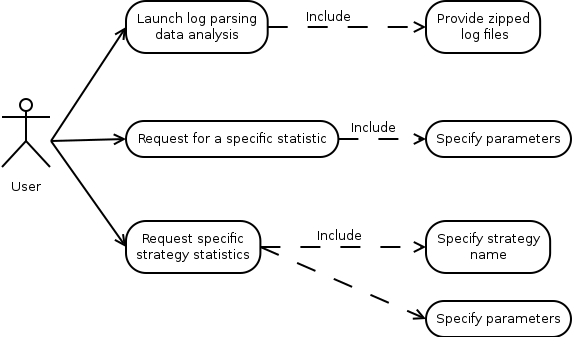
\includegraphics[width=\textwidth,height=\textheight,keepaspectratio]{UseCaseParsing}
\newpage
\textbf{this image shows with more details the use-case of the data analyzes and
data recovery.}\\
\\

\includegraphics[width=\textwidth,height=\textheight,keepaspectratio]{UseCaseDataMining}

\newpage
% 
\includegraphics[width=\textwidth,height=\textheight,keepaspectratio]{UseCaseParser}




\section{The Parser}
% $<$Don’t really say “System Feature 1.” State the feature name in just a few
% words.$>$
This section is dedicated to detail the functional needs of the parser and the
possible problems to be faced on the development of the software.

\subsection{Description and Priority}
% $<$Provide a short description of the feature and indicate whether it is of
% High, Medium, or Low priority. You could also include specific priority
% component ratings, such as benefit, penalty, cost, and risk (each rated on a
% relative scale from a low of 1 to a high of 9).$>$
The parsing will be responsible to read the logs and charge on the database. It
is the highest priority feature as all other functionalities depends on the data
being parsed.

\subsection{Stimulus/Response Sequences}
% $<$List the sequences of user actions and system responses that stimulate the
% behavior defined for this feature. These will correspond to the dialog elements
% associated with use cases.$>$
Where this feature will start automatically on the first run of the program or
be started by the user will be defined on the future (To be decided by the client).

\subsection{The Data}
The data that was provided by the client is compressed in format tar.bz2 , one file for each day of \textit{Log}, the total size of the compressed data is
13Gb.\\
The decompressed data makes a total of 400Gb.
Each \textit{Log} file is in \textit{HTML} format.
A \textit{Log} should contain:
\begin{itemize}
  \item{\textbf{header}} containing the game number and a winner.
  \item{\textbf{match resume}} containing the cards used on the match and how the match
    finished
  \item{\textbf{player resume}} containing each player victory cards, deck and points.UseCaseDataMining
  \item{\textbf{game log}} that part contains all detailed moves made by the players
    during the match
\end{itemize}

\subsubsection{Possibles Issues}
The \textit{Logs} present some data inconsistency that can be problematic on the
development of the parser.
some problems found at the moment that this SRS is being write are:
\begin{itemize}
  \item \textbf{Log number}\\
    The numeration of the logs aren't unique what implies that can't be used to
    identify a log.
  \item \textbf{User Names}\\
    The logs show that no restriction where made on the user names of the game
    and some user names have Keywords and special characters that can conflict
    with the parser.
   \item \textbf{Missing data}\\
     Some of the logs are missing part of the data (like: the header, users
     resume $\ldots$).
   \item \textbf{Log format}\\
     The syntax used to write the logs are not consistent and present some
     difference between logs.
    \item \textbf{Data compression}\\
      As the data is compressed and the equipment provided to work on the
      project can not handle the data uncompressed the project will have to work
      with the compressed data, and after a first benchmark, 4 hours was needed
      to decompress.
\end{itemize}


\subsection{Functional Requirements}
% $<$Itemize the detailed functional requirements associated with this feature.
% These are the software capabilities that must be present in order for the user
% to carry out the services provided by the feature, or to execute the use case.
% Include how the product should respond to anticipated error conditions or
% invalid inputs. Requirements should be concise, complete, unambiguous,
% verifiable, and necessary. Use “TBD” as a placeholder to indicate when necessary
% information is not yet available.$>$

% $<$Each requirement should be uniquely identified with a sequence number or a
% meaningful tag of some kind.$>$

% REQ-1:	REQ-2:
\subsubsection{Read and Store}
Provided the issues revealed by the logs (like: the inconsistency of the syntax)
a use of a parser made with tools like \textit{YACC and LEX} is not recommended.
For that a parser will be done by using the already present \textit{HTML} and
key words presents on the logs.\\

The store of the log data will be done on a NO-SQL database keeping the same
data structure present on the log.\\

The parser is also responsible in working with the compressed data.\\
\newpage
A glimpse of the data to be recognized by the parser is illustrated in this
diagram (some data to be determined as all the possibilities inside a log
haven't being revealed yet):\\

\includegraphics[width=\textwidth,height=\textheight,keepaspectratio]{UseCaseParser}




\subsubsection{database compression}
the database will have to support compression as the client demands that the
size of the database be under 20Gb.


\subsubsection{Tests}

The ideal testing for the parsing would be generate a reverse parser and diff
the original document with the generated one (as proposed by the client).
But provided all inconsistency on the logs creating such test would be really
long, so to make test possible some logs randomly picked will be checked for
lost information manually .


\section{The Analyzer}
% $<$Don’t really say “System Feature 1.” State the feature name in just a few
% words.$>$
This part of the software will be responsible to analyze the data and process
the information generating related statistics and plot charts to easy visualize.


\subsection{Description and Priority}
% $<$Provide a short description of the feature and indicate whether it is of
% High, Medium, or Low priority. You could also include specific priority
% component ratings, such as benefit, penalty, cost, and risk (each rated on a
% relative scale from a low of 1 to a high of 9).$>$
This feature is the high priority of the  project as it is the main
functionality of the program.

\subsection{Stimulus/Response Sequences}
% $<$List the sequences of user actions and system responses that stimulate the
% behavior defined for this feature. These will correspond to the dialog elements
% associated with use cases.$>$
This feature has to parties:
One that will be launched by the user , who will chose/create on type of
analyses and plot.

The other are persistent queries that will be implemented to improve the program
performance, and will be started automatically by the software.


\subsection{Functional Requirements}
% $<$Itemize the detailed functional requirements associated with this feature.
% These are the software capabilities that must be present in order for the user
% to carry out the services provided by the feature, or to execute the use case.
% Include how the product should respond to anticipated error conditions or
% invalid inputs. Requirements should be concise, complete, unambiguous,
% verifiable, and necessary. Use “TBD” as a placeholder to indicate when necessary
% information is not yet available.$>$

% $<$Each requirement should be uniquely identified with a sequence number or a
% meaningful tag of some kind.$>$

% REQ-1:	REQ-2:
In this section the functionalities of the analyzer will be described in
priority order

\subsubsection{ELO}
The first implementation to be made will be the ELO rating system.
More information about ELO cam be found on \url{https://en.wikipedia.org/wiki/Elo_rating_system}
The analyzer will have to calculate the ELO final for each player and what was a
player ELO on a given game.

\subsubsection{Strategies}
The dominion wiki describe some strategies that can be used in the game for
exemple :\\
Big Money\\
Beyond Silver \\
Penultimate Province Rule \\
More on \url{http://wiki.dominionstrategy.com/index.php/Strategy}\\

And the analyzer will have to be able to recognize what strategy was used on a
given match (if any strategy was used) and generate statistics.


\subsubsection{Greening}
The analyzer has to be capable of recognize the \textit{\textbf{greening}} moment on each match.
More about \textit{\textbf{greening}} on \url{http://wiki.dominionstrategy.com/index.php/Greening}

\subsubsection{Charts}
Another function will be the creation of charts based on the analyzed data.
For easy implementation native libraries for plotting charts will be used.

\subsubsection{Queries}
An abstract interface for queries will have to be implemented to give the user
the ability to create his owns analyzes.





\chapter{Nonfunctional Requirements}

\section{Performance Requirements}
% $<$If there are performance requirements for the product under various
% circumstances, state them here and explain their rationale, to help the
% developers understand the intent and make suitable design choices. Specify the
% timing relationships for real time systems. Make such requirements as specific
% as possible. You may need to state performance requirements for individual
% functional requirements or features.$>$
No specific performance requirement was made by the client. But for the analyzer
a time of running should be less than an hour.



\section{reliability}
The client demands that the maximum number of logs should be parsed , as the
data provided has some inconsistencies and some logs wont be possible to parse.
the client agrees that between  5 to 10\% of the logs can be ignored.

The parser will have to parse 100\% of the data present on the log and Restore
any missing information as possible.\\

The data generated by the parser don't need to be human readable.\\

\section{Software Quality Attributes}
% $<$Specify any additional quality characteristics for the product that will be
% important to either the customers or the developers. Some to consider are:
% adaptability, availability, correctness, flexibility, interoperability,
% maintainability, portability, reliability, reusability, robustness, testability,
% and usability. Write these to be specific, quantitative, and verifiable when
% possible. At the least, clarify the relative preferences for various attributes,
% such as ease of use over ease of learning.$>$
Even if just a command line is expected for the final program it should have a
easy learn curve and be easy to use.


%\chapter{Other Requirements}
% $<$Define any other requirements not covered elsewhere in the SRS. This might
% include database requirements, internationalization requirements, legal
% requirements, reuse objectives for the project, and so on. Add any new sections
% that are pertinent to the project.$>$

%\section{Appendix A: Glossary}
% %see https://en.wikibooks.org/wiki/LaTeX/Glossary
% $<$Define all the terms necessary to properly interpret the SRS, including
% acronyms and abbreviations. You may wish to build a separate glossary that spans
% multiple projects or the entire organization, and just include terms specific to
% a single project in each SRS.$>$

%\section{Appendix B: Analysis Models}
% $<$Optionally, include any pertinent analysis models, such as data flow
% diagrams, class diagrams, state-transition diagrams, or entity-relationship
% diagrams.$>$

%\section{Appendix C: To Be Determined List}
% $<$Collect a numbered list of the TBD (to be determined) references that remain
% in the SRS so they can be tracked to closure.$>$

\end{document}
